\section{Resonance Integrals}

%In slowing down, we saw previously that we are concerned with the amount of absorption from some initial (again, monoenergetic) source energy, $E_0$, to the energy of interest, $E$. This is given by:
%\begin{equation*}
%    \int^{E_0}_E \mathrm{d}E'\; \Sigma_\mathrm{a}(E')\phi(E')\;\mathrm{.}
%\end{equation*}
%We return to the resonance escape probability, but we're going to cast it in a more computationall convenient way.The resonance escape probability is defined as:
%\begin{equation*}
%    p(E) = \frac{S_0 - \text{absorption on the way to }E}{S_0} = 1 - \frac{\int^{E_0}_E \mathrm{d}E'\; \Sigma_\mathrm{a}(E')\phi(E')}{S_0}\;\mathrm{.}
%\end{equation*}
%Once again, we want to estimate multigroup cross sections which take the form:
If we cast our minds back to the problem that motivates these lectures, we want to estimate multigroup cross sections of the form:
\begin{equation*}
    \Sigma_{\mathrm{a},g} = \frac{\int^{E_{g-1}}_{E_g}\mathrm{d}E\;\Sigma_\mathrm{a}(E)\phi(E)}{\int^{E_{g-1}}_{E_g}\mathrm{d}E\;\phi(E)}\;\mathrm{.}
\end{equation*}
If we define the \textbf{resonance integral} for resonance $i$ as: 
\begin{equation*}
    I_i = \int_{E_i}\mathrm{d}E\; \sigma^\mathrm{A}_\mathrm{a}(E)\phi(E)\;\mathrm{,}
\end{equation*}
and assert that the resonances are narrow compared to the width of an energy group, $\Delta E_g$, such that $\phi(E) \approx \frac{1}{E}$ (giving $\int^{E_{g-1}}_{E_g}\mathrm{d}E\phi(E) \approx \ln{\frac{E_{g-1}}{E_g}}$), then we can write the cross section as:
\begin{equation*}
    \Sigma_{\mathrm{a},g} = \frac{N_\mathrm{A}\sum_{i\in g}I_i}{\ln{\frac{E_{g-1}}{E_g}}} =\frac{N_\mathrm{A}\sum_{i\in g}I_i 
    }{\Delta u_g}\;\mathrm{.}
\end{equation*}
This means that the problem of calculating cross sections becomes a problem of calculating resonance integrals. This generalises straightforwardly when there is more than one absorbing nuclide. However, this also assumes there is no interference effect between these resonances. We will go through some of the methods used to approximate these integrals in various conditions. This will start from solving the slowing down equation:
\begin{equation}\label{eq:slowing_down}
    \Sigma_\mathrm{t}(E)\phi(E) = \int^{E/\alpha_\mathrm{M}}_E \frac{\Sigma^\mathrm{M}_\mathrm{s}\phi(E')\mathrm{d}E'}{E'(1-\alpha_\mathrm{M})} + \int^{E/\alpha_\mathrm{A}}_E \frac{\Sigma^\mathrm{A}_\mathrm{s}(E')\phi(E')\mathrm{d}E'}{E'(1-\alpha_\mathrm{A})}\;\mathrm{,}
\end{equation}
where we use M to refer to the moderator and A to refer to the resonant absorber.
We make a few approximations:
\begin{itemize}
    \item No absorption in moderator: $\Sigma^\mathrm{M}_\mathrm{t}(E) = \Sigma^\mathrm{M}_\mathrm{s}$.
    \item Only potential scattering in moderator: $\Sigma^\mathrm{M}_\mathrm{s}(E) = \Sigma^\mathrm{M}_\mathrm{s} = \Sigma^\mathrm{M}_\mathrm{p}$.
    \item The absorber cross section can be decomposed as: $\Sigma^\mathrm{A}_\mathrm{t}(E) = \Sigma^\mathrm{A}_\mathrm{a}(E) + \Sigma^\mathrm{A}_\mathrm{s}(E) + \Sigma^\mathrm{A}_\mathrm{p}$.
\end{itemize}
We can make one further approximation in one of two ways, which will affect our results.

\subsection{Narrow resonance approximation}

In this case we first assume that resonances are ``narrow" for collisions with moderator, i.e., $\Gamma_\mathrm{prac}<< \Delta E_\mathrm{M} = \frac{1}{2}(1-\alpha_\mathrm{M})E_0$, or the practical resonance width is much smaller than the average energy loss per collision with moderator. If we make the same assertion for the absorber ($\Gamma_\mathrm{prac}<< \Delta E_\mathrm{M} = \frac{1}{2}(1-\alpha_\mathrm{A})E_0$), this allows us to approximate the flux in the integrals as unperturbed from the asymptotic, i.e., $\phi(E) \sim 1/E$. If we also say the contribution of scattering resonances are also small, then the absorber's scattering cross section is just composed of the potential cross section. Hence, our equations becomes:
\begin{equation*}
     \Sigma_\mathrm{t}(E)\phi_\mathrm{NR}(E) = \int^{E/\alpha_\mathrm{M}}_E \frac{\Sigma^\mathrm{M}_\mathrm{s}\mathrm{d}E'}{E'^2(1-\alpha_\mathrm{M})} + \int^{E/\alpha_\mathrm{A}}_E \frac{\Sigma^\mathrm{A}_\mathrm{p}\mathrm{d}E'}{E'^2(1-\alpha_\mathrm{A})}= \frac{\Sigma^\mathrm{M}_\mathrm{p} + \Sigma^\mathrm{A}_\mathrm{p}}{E}\;\mathrm{,}
\end{equation*}
giving:
\begin{equation*}
    \phi_\mathrm{NR}(E) = \frac{\Sigma^\mathrm{M}_\mathrm{p} + \Sigma^\mathrm{A}_\mathrm{p}}{\Sigma_\mathrm{t}(E)}\frac{1}{E} = \frac{\sigma^\mathrm{A}_\mathrm{p} + \sigma_\mathrm{b}}{\sigma^\mathrm{A}_\mathrm{t}(E) + \sigma_\mathrm{b}}\frac{1}{E}\;\mathrm{,}
\end{equation*}
where $\sigma_\mathrm{b} = \frac{\Sigma_\mathrm{p}}{N^\mathrm{A}}$ is the background cross section. This expression for the flux is known as the narrow-resonance approximation flux -- one thing it implies is that the perturbation due to a resonance depends strongly on the background cross section. This lets us evaluate the resonance integral as:
\begin{equation*}
    I_\mathrm{NR} = \int_{E_0}\mathrm{d}E \sigma^\mathrm{A}_\mathrm{a}(E)\phi_\mathrm{NR}(E) = \int_{E_0}\frac{\mathrm{d}E}{E}\sigma^\mathrm{A}_\mathrm{a}(E)\frac{\sigma^\mathrm{A}_\mathrm{p} + \sigma_\mathrm{b}}{\sigma^\mathrm{A}_\mathrm{t}(E) + \sigma_\mathrm{b}}
\end{equation*}
This can be integrated numerically given we should know how the microscopic cross sections look -- or looked up from a precomputed table given an input background cross section.

We expect the NR approximation to be more valid for higher energy resonances due to the increased average energy loss per collision. %The NR approximation is shown for ... in Fig.~\ref{fig:NR}.

\subsection{Wide resonance approximation}

Also known as the Narrow Resonance-Infinite Mass approximation. This is the other extreme from NR: we say that the average energy loss per collision with an absorber is much less than the practical resonance width, $\frac{1}{2}(1-\alpha_\mathrm{A})E_0 << \Gamma_\mathrm{prac}$. This is illustrated in Fig.~\ref{fig:WR}. As $A\rightarrow\infty$, $\alpha_\mathrm{A}\rightarrow 1$. If we apply this limit to the absorber integral we get:
\begin{equation*}
    \lim_{\alpha_\mathrm{A}\rightarrow 1}\int^{E/\alpha_\mathrm{A}}_E\frac{\mathrm{d}E' \Sigma^\mathrm{A}_\mathrm{s}(E')\phi(E')}{(1-\alpha_\mathrm{A})E'}\rightarrow \Sigma^\mathrm{A}_\mathrm{s}(E)\phi(E)\lim_{\alpha_\mathrm{A}\rightarrow 1} \frac{1}{E}\int^{E/\alpha_\mathrm{A}}_E\frac{\mathrm{d}E'}{1-\alpha_\mathrm{A}} = \Sigma^\mathrm{A}_\mathrm{s}(E)\phi(E)\;\mathrm{.}
\end{equation*}
We use the same $1/E$ treatment for the moderator flux and insert this into the slowing down equation to give:
\begin{equation*}
    \Sigma_\mathrm{t}(E)\phi_\mathrm{WR}(E) = \Sigma^\mathrm{A}_\mathrm{s}(E)\phi_\mathrm{WR}(E) + \frac{\Sigma^\mathrm{M}_\mathrm{s}}{E}\;\mathrm{,}
\end{equation*}
resulting in:
\begin{equation*}
    \phi_\mathrm{WR}(E) = \frac{\Sigma^\mathrm{M}_\mathrm{s}}{\Sigma_\mathrm{t}(E) - \Sigma^\mathrm{A}_\mathrm{s}(E)}\frac{1}{E} = \frac{\sigma_\mathrm{b}}{\sigma^\mathrm{A}_\mathrm{a}(E) + \sigma_\mathrm{b}}\frac{1}{E}\;\mathrm{.}
\end{equation*}
Once again, this can be used to evaluate resonance integrals, dependent on the background cross section.

\begin{figure}[h]
  \centering
  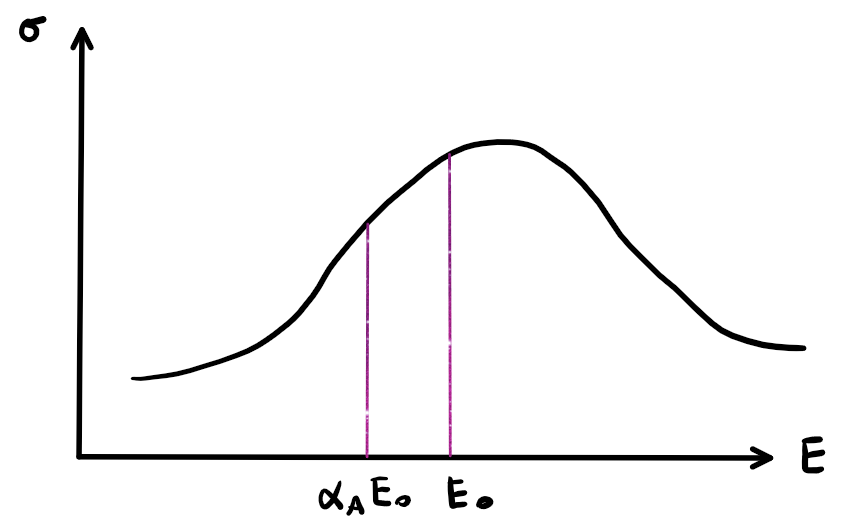
\includegraphics[scale=0.60]{./Figures/P4/scatterWR.png} 
  \caption{Illustration of the wide resonance approximation.} 
  \label{fig:WR}
\end{figure}
From both the NR and WR approximations, if the background cross section (or dilution) is very high, we would obtain the infinite dilution resonance integral:
\begin{equation*}
    I^\infty = \int_{E_0}\mathrm{d}E \sigma^\mathrm{A}_\mathrm{a}(E)\frac{1}{E}\;\mathrm{.}
\end{equation*}
Note that $I^\infty > I_\mathrm{NR}$ and $I^\infty > I_\mathrm{WR}$. This is the effect of self-shielding!

\subsection{Intermediate resonance approximation}

The difference between the NR and WR approximations is ultimately whether we include contributions from the scattering cross section of the resonant nuclide. This suggests that we can do something part-way, i.e., have an \textbf{intermediate} resonance approximation where we only include part of the scattering cross section. This is done with a parameter $\lambda$ such that we have:
\begin{equation*}
    \phi_\mathrm{IR}(E) =  \frac{\lambda\sigma^\mathrm{A}_\mathrm{p} + \sigma_\mathrm{b}}{\sigma^\mathrm{A}_\mathrm{a}(E) + \lambda\sigma^\mathrm{A}_\mathrm{p} +  \sigma_\mathrm{b}}\frac{1}{E}\;\mathrm{,}
\end{equation*}
where $\lambda$ is a parameter deciding the importance of the scattering cross section for a particular resonance; $\lambda =1$ corresponds to NR, $\lambda=0$ corresponds to WR. This model tends to produce significantly better results in intermediate energy ranges where neither the narrow nor wide approaches are very accurate. As such, it is commonly used in many lattice physics codes. However, the determination of the $\lambda$ parameters for a given system is not elegant -- this is usually done numerically and fixed for future use.
